\chapter{Implementation and Results}
\label{implementation}
In this chapter, we test our system and discuss the results. First, we illustrate how the simulation is carried out, and then, we explain our methodology to test PIVOT, defining the parameters and how they affect the simulations. 

\section{Implementation}
\label{simulator}
\begin{figure}[H]
    \centering
    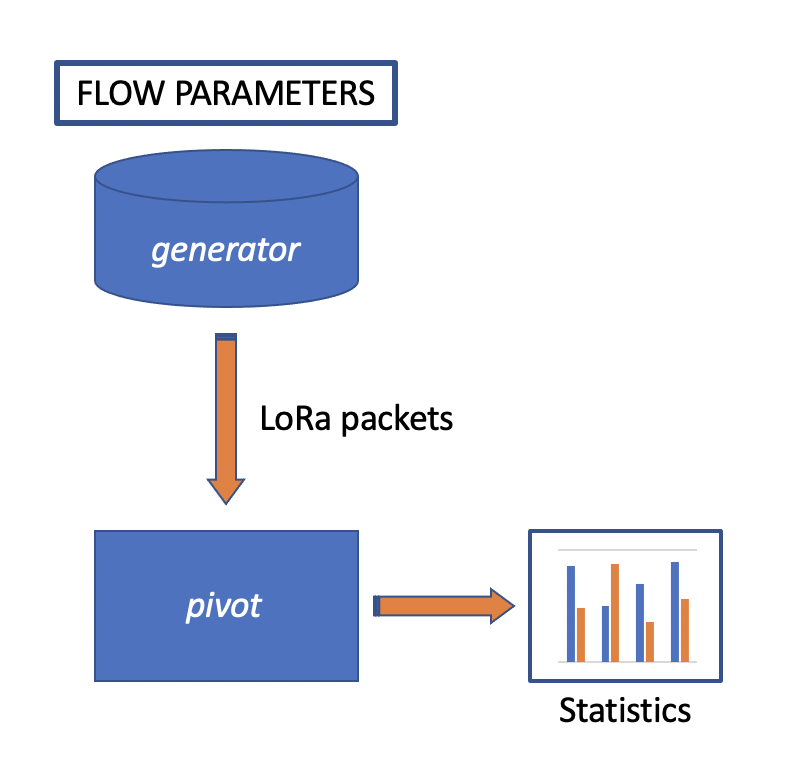
\includegraphics[width=0.5\linewidth]{images/implementation/simulator.png}
    \caption{The architecture of the simulator}
    \label{fig:simulator}
\end{figure}
PIVOT is tested by running it in a simulated LoRaWAN network. As shown in figure \ref{fig:simulator}, the simulator is made up of two components, the \textit{generator} and \textit{pivot}. The LoRa traffic is set and created by the \textit{generator} to be subsequently read and analyzed by \textit{pivot}. In detail, the \textit{generator} takes as input a set of parameters that determine the characteristics of the flow, such as the number of devices generating packets or the transmission frequency. On the other side, \textit{pivot} outputs the list of statistics metrics, described in Chapter \ref{pivot}. The simulation program was created using Python 3.7 and its source code is fully observable and downloadable from Github \cite{terenzi}.

\subsection{Code description}
In this section we analyze in detail the \textit{generator} and \textit{pivot} components, displaying code snippets where relevant.

\subsubsection{\textit{generator}}
The generator subroutine outputs a synthetic LoRa dataset, whose components are instances of the \texttt{Packet} class, shown in the following snippet.

\vspace{3mm}
\begin{mintedbox}[samepage]{python}
class Packet:
	def __init__(self, t, dev, devaddr, rssis, uid, fcnt, mtype, info=""):
		self.rssis = rssis  #can be None, if unavailable
		self.dev_eui = dev
		self.dev_addr = devaddr
		self.t = t
		self.uid = uid
		self.fcnt = fcnt
		self.mtype = mtype
		self.info = info
\end{mintedbox}

\vspace{3mm}

The class variables are well-known LoRa header fields, such as the two identifiers, the DevAddr and the DevEUI, the Message type \textit{mtype} and the timestamp \textit{t}.
\\
In the original LoRaWAN specification there are six different message types, differently codified in the \textit{mtype} fields. Since PIVOT filters only \textit{uplink} and \textit{Join-request} messages, the sole ones required, our simulator avoids generating unnecessary messages. The \textit{mtype} of packets in the dataset are set exclusively to \texttt{000} (Join-request) and \texttt{010} (Unconfirmed Data Up). Moreover, LoRaWAN requires encrypting the payload using AES. Since the covered information cannot be read by external parts, such as PIVOT, we decide to omit this field in the class.
\\
The DevAddress and DevEUI parameters also have a slightly different syntax from the official guidelines. The value of the DevEUI is given by an index \(\ i \) used to represent the device \(\ i \)-th in the simulated network. The DevAddress is the concatenation of the DevEUI and the \(\ j \) index, a counter that indicates the number of Join-request messages sent by the \(\ i \)-th device.
\\
These measures are conceived to forge packets containing only essential elements for our purposes. Smaller packets imply large datasets to use in our tests.

\vspace{3mm}
\begin{mintedbox}{python}
N = 300     # number of devices
S = 365*24*3600     # number of seconds to generate packets
Tmin = int(10)      # minimum interarrival time, in seconds
Tmax = int(23*3600)     # maximum interarrival time, in seconds
Emin = 0.01     # minimum absolute error in the interarrival time, in seconds
Emax = 2        # maximum absolute error in the interarrival time, in seconds
P = 10      # maximum length of a pattern
Jmin = 20       # minimum number of messages before a join
Jmax = 300      # maximum number of messages before a join
\end{mintedbox}
\vspace{3mm}

The code above reports the set of parameters used to determine the characteristics of the traffic flow. The first variable to note is \(\ N \), the number of \textit{active} devices in the network i.e. all that endpoints that from the moment PIVOT is turned on send at least one frame in the network. \(\ N \) implicitly also represents the maximum number of devices that our system can detect. In the best scenario, given the vector \(\ C \) used by PIVOT to store all the identified patterns, we have \(\ length(C) = N \).
\\
The parameter \(\ P \) represents the maximum length of the pattern i.e. the number of segments \(\ s_{1}, ..., s_{n} \) that compose the chain while \(\ Tmin \) and \(\ Tmax \) are respectively the smallest and the largest values that the segment \(\ s \) can take.
\\
Using with three keys, the generator elaborates a new random pattern in this way:

\vspace{3mm}
\begin{mintedbox}{python}
# generate random pattern for the current device
pattern_len = randint(1, P)
pattern = [randint(Tmin, Tmax) for _ in range(pattern_len)]
\end{mintedbox}
\vspace{3mm}

To make the fake traffic as likely as possible to the real one, the simulator inserts a small error during the creation of packets. The system doesn't rigidly generate new packets following the established pattern, but supposes that the time distance between two messages (i.e. a \textit{segment}), could be longer or shorter than expected. Then, it randomly chooses an error \(\ E \) in the range \(\ [Emin, Emax] \) alters slightly the segment in the following way:

\vspace{3mm}
\begin{mintedbox}{python}       
# generate packets following the pattern up until S seconds
packets_dev = []
i_pattern = 0
t = first_packet_t
while t < S:
    packets_dev.append(next_packet)
    t_err = (1.0 if random()>0.5 else -1.0) * (random() * (Emax - Emin) + Emin)
    # It could be the case that t_err is negative and |t_err| > pattern[i_pattern].
    # In this case the following assert yields an error
    next_packet_t = t + pattern[i_pattern] + t_err
    if t_err < 0 and abs(t_err) > abs(pattern[i_pattern]):
        # next_packet_t is set to be 10 seconds after the previous one
        next_packet_t += abs(t_err) - abs(pattern[i_pattern]) + 10
    assert(next_packet_t > t)
    next_packet = Packet(next_packet_t, str(dev_i), "---", None, None, -1, "Unconfirmed Uplink")

    i_pattern = (i_pattern+1) % pattern_len
    t = next_packet_t
\end{mintedbox}
\vspace{3mm}

Finally, we introduce the last two parameters, \textit{Jmin} and \textit{Jmax}, the minimum and the maximum number of messages before a join. They are a keystone for the correct functioning of PIVOT as they influence the accuracy of the detection algorithm. Indeed, if a device sends many packets before sending a \textit{Join-request}, the probability that the system identifies its pattern is very high.

\vspace{3mm}
\begin{mintedbox}{python}       
# add join messages for the current device
joins_dev = []
i = randint(Jmin, Jmax)
while i < len(packets_dev)-1:
    t1 = packets_dev[i].t
    t2 = packets_dev[i+1].t
    assert(t2 > t1)
    join_msg_t = t1 + (random() * (t2-t1))
    assert(t1 < join_msg_t < t2)
    join_packet = Packet(join_msg_t, str(dev_i), "not_available", None, None, -1, "Join Request")
    joins_dev.append(join_packet)
    i += randint(Jmin, Jmax)
\end{mintedbox}
\vspace{3mm}

\subsubsection{\textit{patterns}}
The following code snippet reports the constructor of the \texttt{Pattern} class. As reported in Chapter \ref{pivot}, PIVOT stores each detected pattern along with the last \(\ timestamp \), the chain of \(\ segments \) and the \(\ verified \) flag, initialized to False.

\vspace{3mm}
\begin{mintedbox}[samepage]{python}
class Pattern:
    def __init__(self, timestamp):
        self.timestamp = timestamp
        self.verified = False
        self.segments = []
\end{mintedbox}
\vspace{3mm}

Each element in the chain of segments is an instance of the \texttt{Segment} class. In detail, a segment \(\ s \) is stored with a counter \(\ n \) and an value \(\ mean \), two parameters used to reduce the percentage of errors in defining the exact length of the segment.

\vspace{3mm}
\begin{mintedbox}[samepage]{python}
class Segment:
    def __init__(self, value, index):
        self.n = 1
        self.index = index
        self.mean = value
\end{mintedbox}
\vspace{3mm}

As we have seen previously, a device does not always strictly follow its pattern, sending sometimes packets a little earlier or later than required. Then, the \(\ mean \) represents the average size, in seconds, of the segment \(\ s \) in a given pattern.

\vspace{3mm}

Going into details, for each new DevAddress \(\ a \), PIVOT initialize an empty pattern \(\ P_{a} \). Then, when it receives a new packet \(\ p \) with the DevAddress \(\ a \), it triggers the \textit{update} subroutine:

\vspace{3mm}
\begin{mintedbox}{python}
def update(self, timestamp):
    old_t = self.timestamp 
    self.timestamp = timestamp
    x = self.timestamp - old_t
    
    found = False
    for s in self.segments:
        if abs(s.mean - x) < e:
            found = True
            s.update(x) 
    
    if found:
        self.verified = True

    if not found:
        # new segment
        index = len(self.segments) - 1
        segment = Segment(x, index)
        self.segments.append(segment)
        self.verified = False
\end{mintedbox}
\vspace{3mm}

This function calculates the current segment \(\ s \), checks if it is in the chain of the pattern, and, if needed, updates the flag \textit{verified}. In observing that the segment already belongs to the chain, the algorithm considers a possible margin of error \(\ e \). When the assertion is verified, PIVOT triggers the method \(\ update \) of the class \texttt{Segment}:

\vspace{3mm}
\begin{mintedbox}{python}
def update(self, value):
    self.n += 1
    old_m = self.mean
    self.mean = old_m + ((value - old_m) / self.n)
\end{mintedbox}
\vspace{3mm}

This procedure is used to level the value of the \textit{mean} parameter so that, despite the errors in the transmission, it can remain as accurate as possible to the real length of the segment. The updated value is the outcome of Welford's online algorithm \cite{welford}, which computes the mean in a single pass, inspecting each value only once.

\vspace{3mm}

The last method of the \texttt{Pattern} class we are going to describe is \textit{equals}, which code is reported below:

\vspace{3mm}
\begin{mintedbox}{python}       
def equals(self, pattern):

    if len(pattern.segments) != len(self.segments):
        return False

    segments = pattern.segments
    for s in segments:
        if not s.belongs_to(self):
            return False
    
    return True
\end{mintedbox}
\vspace{3mm}

This procedure verifies a matching between two patterns \(\ P_{1} \) and \(\ P_{2} \). They are equal when the two chains are of the same length, with the same number of segments of equal length, sequentially distributed in the same way. When all these requirements are confirmed, the function returns \texttt{True}.

\subsubsection{\textit{pivot}}
The following snippet displays the constructor of the \texttt{PIVOT} class:
\begin{mintedbox}[samepage]{python}
class PIVOT:
    def __init__(self):
        self.confirmed = {}
        self.unconfirmed = {}
        self.quarantine = {}

        self.to_analyze = {}
        self.current_section = 1
\end{mintedbox}
The \textit{confirmed}, \textit{unconfirmed}, and \textit{quarantine} variables represent the \(\ C \), \(\ U \), and \(\ Q \) vectors described in Chapter \ref{pivot}. These Python dictionaries stores the couples <dev\_addr, pattern>, where "dev\_addr" is the well-known identifier of the device and "pattern" is an instance of the Pattern class associated with the DevAddress. In detail, \textit{confirmed} contains all the unique patterns detected by PIVOT, \textit{unconfirmed} collects all the undetected ones i.e. associated with devices not yet recognized and finally \textit{quarantine} has all that patterns that matches with almost one of those that are in \textit{confirmed}.
\\
\textit{to\_analyze}, that represent the data structure \(\ TA \), stores the pairs <dev\_addr, list\_to\_analyze>, where the key "dev\_addr" is an unknown DevAddress, which pattern P is in \textit{unconfirmed}, and "list\_to\_analyze" is a list of candidate patterns to compare with P.
\\
Finally, \textit{current\_section} is a counter used to estimate the number of section i.e. the amount of intervals between two Join-requests.

\vspace{3mm}

After the initialization of PIVOT, to simulate an incoming data stream, the dataset outputted by the \textit{generator} is processed through a for loop, within which the \textit{read\_packet} method is triggered.

\vspace{3mm}
\begin{mintedbox}{python}
# generating the dataset
generate_synt_traffic(400)

# loading the dataset
packets =  pickle.load(open("synth_traffic.pickle", "rb"))

# new instance of PIVOT
pivot = PIVOT()

# PIVOT on listening
# analyzing the dataset
for p in packets:
    pivot.read_packet(p)
\end{mintedbox}

\vspace{3mm}

The function \textit{read\_packet} processes the incoming packet, extracting and analyzing the \texttt{mtype} field. As long as this value is different from "Join Request" and the current section is \(\ 1 \), PIVOT triggers the internal \textit{pre\_join} subroutine. Otherwise, it calls the \textit{main} one.

\vspace{3mm}
\begin{mintedbox}{python}
def read_packet(self, p):
    if (p.mtype == "Join Request"):
        self.current_section += 1

    else:
        if self.current_section == 1:
            self.__pre_join(p)
        else:
            self.__post_join(p)  
\end{mintedbox}
\vspace{3mm}

The \textit{pre\_join} function is a subroutine of the detection algorithm. As explained in Chapter \ref{pivot}, in this step the first patterns are identified and modeled, to be subsequently used as a
reference in the \textit{main} procedure. When the current DevAddr is not a key of the \textit{confirmed} dictionary, a new instance of the \texttt{Pattern} class is triggered. When instead it is a key, the associated pattern is extracted and updated triggering the \textit{update} method of the \texttt{Packet} class.

\vspace{3mm}
\begin{mintedbox}[samepage]{python}
def __pre_join(self, p):
    devaddr = p.dev_addr

    if devaddr in self.confirmed:
        self.confirmed[devaddr].update(p.t)
    else:
        self.confirmed[devaddr] = Pattern(p.t)
\end{mintedbox}
\vspace{3mm}

When the function \textit{read\_packet} processes an uplink packet and the current section is greater than \(\ 1 \), it calls the internal \textit{main} subroutine. This procedure analyzes the DevAddress and checks progressively if it a key of the \textit{confirmed} dictionary or of the \textit{unconfirmed} one.
\vspace{3mm}
\begin{mintedbox}{python}
def __main_procedure(self, p):
    
    # gets the Dev Address
    devaddr = p.dev_addr  
    
    # checks if the pattern already exists
    if devaddr in self.confirmed:
        self.confirmed[devaddr].update(p.t)
        self.__clean(devaddr)

    else:
        # check if the DevAddress has already been received
        if devaddr in self.unconfirmed:
            self.unconfirmed[devaddr].update(p.t)
            
            # checks if the DevAddress is in Quarantine
            if devaddr in self.quarantine:
                self.__quarantine(devaddr, p.t)

            else:
                # cheks if the pattern associated with the DevAddress matches with other patterns 
                to_analyze = self.to_analyze[devaddr]
                unconf_pattern = self.unconfirmed[devaddr]


                verified = list(filter(lambda x: self.confirmed[x].verified, to_analyze))

                for v in verified:
                    conf_pattern = self.confirmed[v]        

                    if len(unconf_pattern.segments) == len(conf_pattern.segments):
                        pattern_matching = conf_pattern.contains(unconf_pattern)
                    
                        if pattern_matching:
                            # there is a match, the DevAddress is put in Quarantine        
                            self.quarantine[devaddr] = (v, p.t)      
                        else:
                            self.to_analyze[devaddr].remove(v)

                if len(self.to_analyze[devaddr]) == 0:
                    self.__new_device(devaddr, unconf_pattern)   

        else:
            # initializing a new pattern
            self.unconfirmed[devaddr] = Pattern(p.t)
            self.to_analyze[devaddr] = list(self.confirmed.keys()
\end{mintedbox}
\vspace{3mm}

If neither of these two conditions occurs, the DevAddress belongs to an unknown device. PIVOT creates a new instance of \texttt{Pattern}, inserts it in the \textit{unconfirmed} dictionary, and sets the \textit{to\_analyze} list with all the potential patterns with which it must verify the match. Initially, this list is filled with all the keys of the \textit{confirmed} dictionary.

\vspace{3mm}

Otherwise, if the DevAddress is a key of the \textit{confirmed} dictionary, it belongs to a device that did not make any Join-request, and then, did not change its address. This scenario implies that the associated pattern should not used as comparison model for other patterns. The \textit{clean} function is triggered. 

\vspace{3mm}
\begin{mintedbox}{python}
if devaddr in self.confirmed:
    self.confirmed[devaddr].update(p.t)
    self.__clean(devaddr)
\end{mintedbox}

\vspace{3mm}

This method simply removes from all the \textit{to\_analyze} lists the value \(\ devaddr \) given as input.

\vspace{3mm}
\begin{mintedbox}{python}
def __clean(self, devaddr):
    to_analyze = self.to_analyze.copy()

    for elem in to_analyze:
        if devaddr in to_analyze[elem]:
            self.to_analyze[elem].remove(devaddr)
\end{mintedbox}

\vspace{3mm}

Now, we analyze the case where the DevAddress is a key of the \textit{unconfirmed} dictionary. First of all, PIVOT check if this address belongs to the \textit{quarantine} dictionary also and, eventually, triggers the quarantine subroutine. Otherwise, it starts the matching procedure. It takes all the addresses stored in \textit{to\_analyze[DevAddress]} and extracts their respective patterns from \textit{confirmed}. To ensure greater accuracy, only those patterns whose \textit{verified} flag is set to \texttt{True} are taken into account. This newly obtained list is analyzed through a for loop. For simpler notation, we denote the pattern of the unconfirmed DevAddr as \texttt{unconf\_pattern} and the current verified pattern we are going to compare with as \texttt{conf\_pattern}. When there is a matching between the two patterns, their respective DevAddress are inserted in the \textit{quarantine} dictionary so that the next time a new packet arrives with that DevAddress, PIVOT will trigger the \textit{quarantine} subroutine. In all other cases where there is no match, the \textit{to\_analyze} list is updated, removing from it the address associated to the current \texttt{conf\_pattern}.

\vspace{3mm}
\begin{mintedbox}{python}
if devaddr in self.unconfirmed:
    self.unconfirmed[devaddr].update(p.t)
    
    if devaddr in self.quarantine:
        self.__quarantine(devaddr, p.t)

    else:
        to_analyze = self.to_analyze[devaddr]
        unconf_pattern = self.unconfirmed[devaddr]


        verified = list(filter(lambda x: self.confirmed[x].verified, to_analyze))

        for v in verified:
            conf_pattern = self.confirmed[v]        

            if len(unconf_pattern.segments) == len(conf_pattern.segments):
                pattern_matching = conf_pattern.contains(unconf_pattern)
            
                if pattern_matching:
                    self.quarantine[devaddr] = (v, p.t)      
                else:
                    self.to_analyze[devaddr].remove(v)

        if len(self.to_analyze[devaddr]) == 0:
            self.__new_device(devaddr, unconf_pattern)  
\end{mintedbox}
\vspace{3mm}

At the end of the loop, if the \textit{to\_analyze} list is empty, then \texttt{unconf\_pattern} hasn't had any matches and necessarily it is linked to a new device. PIVOT calls the function \textit{new\_device}, that registers the \texttt{unconf\_pattern} in the \textit{confirmed} dictionary and updates all the data structures, removing the DevAddress from \textit{unconfirmed} and deleting the \textit{to\_analyze} list.

\vspace{3mm}
\begin{mintedbox}{python}
def __new_device(self, devaddr, unconf_pattern):
    self.confirmed[devaddr] = unconf_pattern
    self.unconfirmed.pop(devaddr)
    self.to_analyze.pop(devaddr)
\end{mintedbox}

\vspace{3mm}

Finally, we illustrate the \textit{quarantine} subroutine, reported in the following snippet. This procedure takes as input the variable \texttt{devaddr} i.e. the unknown DevAddress of which we must identify the device, and triggers an alarm if it detects that \texttt{devaddr} belongs an already joined device. The \textit{quarantine} makes use of two parameters, \texttt{pattern}, that represent the pattern that matches with the one associate to \texttt{devaddr}, and \texttt{suspect}, that is the DevAddress correlated to \texttt{pattern}.
\\
This function first calculates the current segment associated to \texttt{devaddr}, then checks if it is in the chain of \texttt{pattern}. In that case, we have the confirm that the \texttt{suspect} and the \texttt{devaddres} belong to the same device. The alarm is triggered and the \textit{confirmed} dictionary is updated, replacing the key \texttt{suspect} with \texttt{devaddr} since it is the current address of that device. Moreover, the function \textit{clean} is called so that the variable \texttt{suspect} is removed from the \textit{to\_analyze} lists (therefore it will no longer be taken into consideration in the matching procedures).
\\
On the other hand, if the segment don't belong to the chain of \texttt{pattern}, the variable \texttt{devaddr} represents a new device, and it is added as a new key in \textit{confirmed}.

\vspace{3mm}
\begin{mintedbox}{python}
def __quarantine(self, devaddr, p_timestamp):
    suspect = self.quarantine[devaddr][0]
    timestamp = self.quarantine[devaddr][1]
    pattern = self.confirmed[suspect]

    x = Segment(p_timestamp - timestamp, 0)
    if x.belongs_to(pattern):
        self.confirmed[devaddr] = self.unconfirmed[devaddr]
        self.confirmed.pop(suspect)
        self.__clean(suspect)

    else:
        new_pattern = self.unconfirmed[devaddr][suspect]
        self.confirmed[devaddr] = new_pattern

    self.unconfirmed.pop(devaddr)
    self.quarantine.pop(devaddr)
    self.to_analyze.pop(devaddr)
\end{mintedbox}
\vspace{3mm}

At the end of \textit{quarantine}, since PIVOT has successfully identified the nature of \texttt{devaddr}, it removes it from \textit{unconfirmed}, \textit{quarantine} and \textit{to\_analyze} structures.

\vspace{3mm}

\subsubsection{metrics for the operator}
The following snippet reports the four metrics that PIVOT outputs to the operator.
\vspace{3mm}
\begin{mintedbox}{python}
def metrics(self):
    number_of_unique_devices = len(self.confirmed)
    number_of_detected_devices = self.detected
    return {
        "NoUD" : len(self.confirmed),
        "NoJ" : self.current_section - 1,
        "NoDD": self.detected,
        "PoDD" : number_of_detected_devices / number_of_unique_devices
    }
\end{mintedbox}
\vspace{3mm}

\newpage

\section{Results}
\label{results}
In this section, we show the results of the various tests carried out using the simulator. In particular, we first analyze the \textit{sensitivity} of PIVOT, showing which parameters can affect the correct functioning of the system. Subsequently, we will compare two different scenarios to demonstrate how by applying countermeasures described in Chapter \ref{pivot} the operator can effectively reduce the vulnerability of exposed devices. All the evaluations are run with Python3.7 on a x64 laptop equipped with a Intel Core i7 CPU @2.50GHz and 8 GB of RAM.

\subsection{Sensitivity of the system}
Basic performance measures can be derived from the \textit{confusion} matrix, shown in figure \ref{fig:classification}. It is a two-by-two table containing four outcomes produced by a binary classifier, used to derive well-known statistical criteria, such as error rate, accuracy, specificity, sensitivity, and precision.

\vspace{3mm}
\begin{figure}[H]
    \centering
    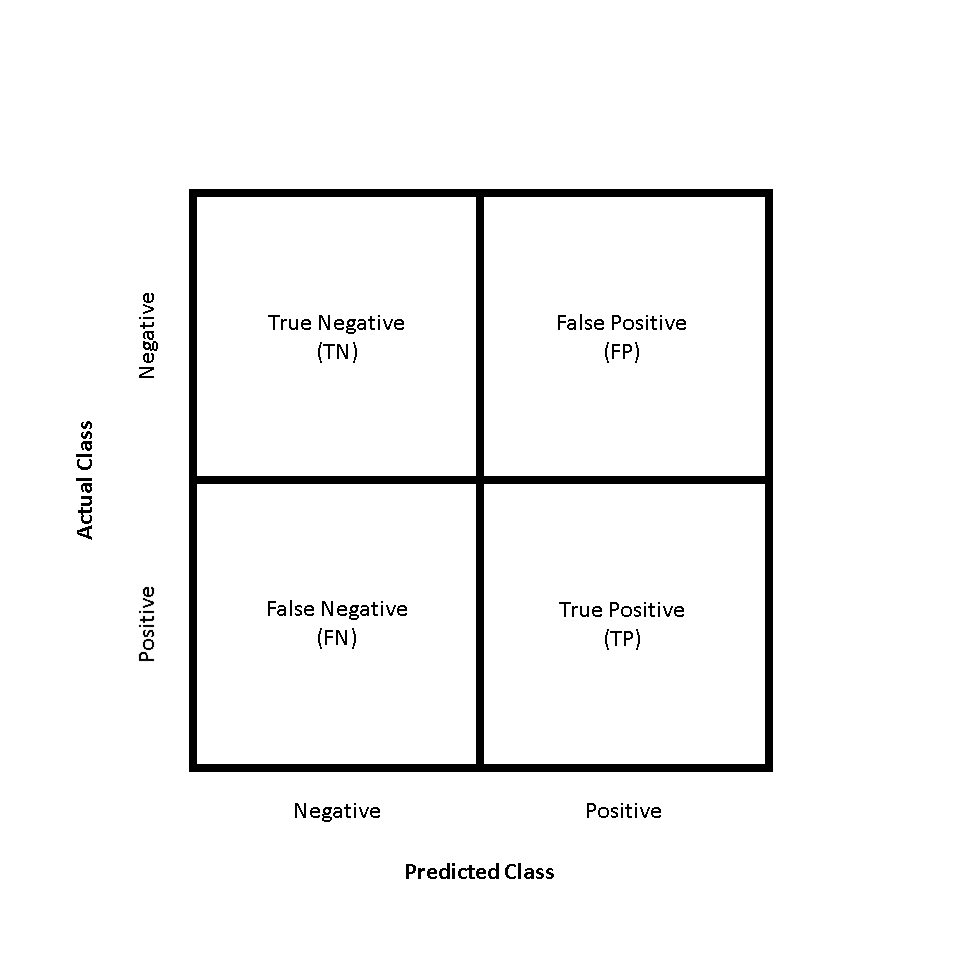
\includegraphics[width=0.7\linewidth]{images/implementation/binary_classification.png}
    \caption{Confusion matrix structure for binary classification problems}
    \label{fig:classification}
\end{figure}
\vspace{3mm}

For our tests, we define the \textit{positive} and \textit{negative } classes in this way:

\vspace{3mm}
\begin{itemize}
    \item The \textbf{positive} class represents the number of times in which devices, sending a Join-request, change their DevAddress. This value can also be interpreted as the total number of times PIVOT could potentially recognize a match between two patterns.
    \item The \textbf{negative} class is the number of ED that have never changed their address. PIVOT should be able to classify them as \textit{new} devices. 
\end{itemize}
\vspace{3mm}

Going into detail, in a binary classification like the one just described, there are four possible outcomes.

\vspace{3mm}
\begin{itemize}
    \item \texttt{True positive (TP)}: correct positive prediction
    \item \texttt{False positive (FP)}: incorrect positive prediction
    \item \texttt{True negative (TN)}: correct negative prediction
    \item \texttt{False negative (FN)}: incorrect negative prediction
\end{itemize}

\vspace{3mm}

According to the positive and negative classes defined above, these four metrics can be interpreted in the following way:

\vspace{3mm}
\begin{itemize}
    \item \texttt{True positive (TP)}: PIVOT recognizes a match between two patterns and they belongs to the same ED.
    \item \texttt{False positive (FP)}: PIVOT recognizes a match between two patterns but they belongs to different EDs.
    \item \texttt{True negative (TN)}: PIVOT correctly classifies a DevAddr as belonging to a new device. 
    \item \texttt{False negative (FN)} : PIVOT classifies a DevAddr as belonging to a new device, but it is an already joined device that changes its address. 
\end{itemize}
\vspace{3mm}

From these values, we can compute the \texttt{True Positive Rate (TPR)}, commonly known as sensitivity or recall. The technical definition of TPR is the number of true positives divided by the number of true positives plus the number of false negatives.

\[ TRP = \frac{TP}{TP + FN} \]

In other words, it represents the ability our model to find all the relevant matches within the data set and, if compared to other more well-known metrics, such as accuracy, it allows us to draw more specific conclusions from the various tests. Indeed, despite accuracy being a more intuitive performance measure, it is simply a ratio of correctly predicted observations to the total observations and works better with symmetric datasets where the number of false positive and false negatives are almost the same. Imbalanced classification tasks requires more sophisticated statistical parameters such as precision and, precisely, recall, from the combination of which it is possible to obtain useful models, such as the F1 score.

\vspace{3mm}
\begin{table}[H]
    \caption{The two variables used to analyze the sensitivity of the detection algorithm.}
    \label{tab:parameters}
    \centering
    \begin{tabular}{|c|l|}
    \hline
    \textbf{Parameter} & \textbf{Description}             \\ \hline
    \texttt{N}         & Number of active devices in the network \\ \hline
    \texttt{P}         & Maximum length of patterns       \\ \hline
    \end{tabular}
\end{table}
\vspace{3mm}

Given the definition of recall, we now illustrate how the different parameters can influence the value of this metric. Table \ref{tab:parameters} reports the two variables we choose to determining the characteristics of the traffic generated by the simulator. In the following tests, we use them to analyze the sensitivity of the PIVOT detection algorithm by varying a chosen variable and fixing the remaining one to predetermined values.

\vspace{3mm}

\subsubsection{Parameter N}
The first variable in analysis is \(\ N \), the overall number of \textit{active} devices in the network i.e. all that ED that sends almost one packet while PIVOT is running. In detail we conducted 31 different measurements, ranging the value of \(\ N \) from 50 to 200, with an increment of 5 after each iteration. The figure \ref{fig:testn} reports the results of the evaluation:

\vspace{3mm}
\begin{table}[H]
\centering
\caption{The value of the parameters used to generate the traffic flow for this test.}
\label{tab:parameter_N}
\begin{tabular}{|l|l|}
\hline
\multicolumn{1}{|c|}{\textbf{Parameter}} & \textbf{Value} \\ \hline
N                                        & Variable            \\ \hline
P                                        & 5              \\ \hline
J                                     & [20, 300]             \\ \hline
E                                     & [0.01, 2]           \\ \hline
\end{tabular}
\end{table}
\vspace{3mm}

\vspace{3mm}
\begin{figure}[H]
    \centering
    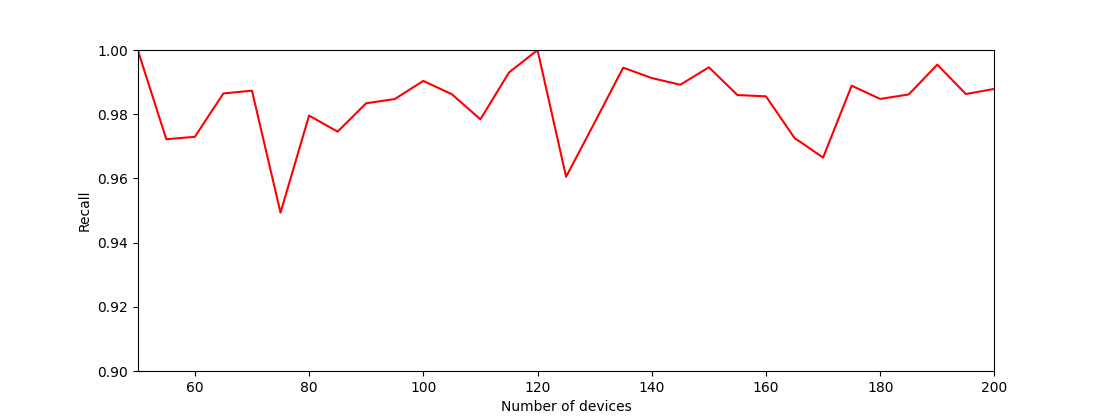
\includegraphics[width=1\linewidth]{images/implementation/N.png}
    \caption{This figure shows the recall value as parameter N changes. The sensitivity of the system scales from from the lowest 0.94 to the highest 1.0, with an average value of 0.98}
    \label{fig:testn}
\end{figure}
\vspace{3mm}

The recall ranges from the lowest 0.94 to the highest 1.0, with an average value of 0.98. This small range of values demonstrates that PIVOT identifies almost all vulnerable devices regardless of the number of endpoints in the network.

\vspace{3mm}

\subsubsection{Parameter P}
Now we analyze how recall varies according to parameter \(\ P \), the maximum length that a pattern can have within the network. We tested 29 different scenarios, with a value of \(\ P \) ranging from a minimum of 2 to a maximum of 30.

\vspace{3mm}
\begin{table}[H]
\centering
\caption{The value of the parameters used to generate the traffic flow for this test.}
\label{tab:parameter_P}
\begin{tabular}{|l|l|}
\hline
\multicolumn{1}{|c|}{\textbf{Parameter}} & \textbf{Value} \\ \hline
N                                        & 100            \\ \hline
P                                        & Variable              \\ \hline
J                                     & [20, 300]             \\ \hline
E                                     & [0.01, 2]           \\ \hline
\end{tabular}
\end{table}
\vspace{3mm}

\vspace{3mm}
\begin{figure}[H]
    \centering
    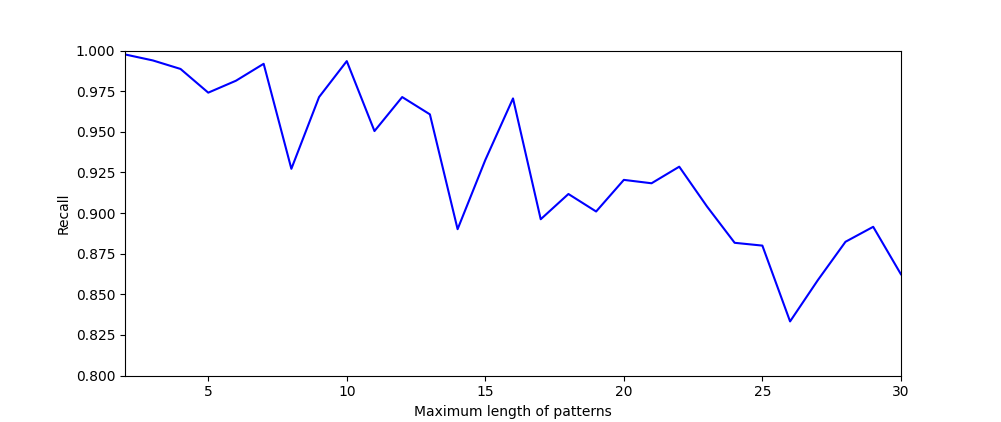
\includegraphics[width=1\linewidth]{images/implementation/P.png}
    \caption{This figure shows the recall value as parameter P changes. The sensitivity of the system scales from a minimum of 0.83 to a maximum of 0.99, with a mean of 0.92}
    \label{fig:testp}
\end{figure}
\vspace{3mm}

In this case, the results scales from a minimum of 0.83 to a maximum of 0.99, with a mean of 0.92. However, as shown in figure \ref{fig:testp}, the detection algorithm is less effective as the length of the pattern increases. Indeed, PIVOT takes longer to recognize complex patterns, consequently leaving many addresses waiting to be classified. In any case, the effectiveness of the algorithm does not experience strong changes in the presence of shorter patterns. And since most LoRaWAN devices have just this kind of patterns, this represents an advantage.

\vspace{3mm}


\subsection{Testing the countermeasures}
In this section we show that the strategies explained in Chapter \ref{pivot} can effectively increase the security level of a LoRaWAN network. In detail, our demonstration consists of two steps. First, we generate and analyze a normal LoRa traffic flow then, we alter the inter-arrival time between packets by adding an \textit{exponential delay}, and, finally, we use the metrics produced by PIVOT to compare the two scenarios.

\vspace{3mm}

The following code snippet reports the \textit{add\_exp\_delay} function, used by the generator to change the traffic flow (represented by the dataset \texttt{patterns}) given in input.

\vspace{3mm}
\begin{mintedbox}{python}
def add_exp_delay(packets, exp_rate):
    assert(exp_rate>0)

    # total delay of all the packets, in seconds
    exp_total_delay = 0
    # list percentual increases of the delay
    exp_delay_inc = []
    # number of exponential arrival not used. An exponential arrival is not used if it arrives before the original interarrival time of the packet
    exp_total_notused = 0

    devs = set([p.dev_eui for p in packets])  #set of all devices
    
    for dev in devs:
        packets_dev = [p for p in packets if p.dev_eui == dev]
        
        # init exponential interarrival times generator
        exp_gen = exp_generator(exp_rate)

        # modify packet arrival times
        t_exp = packets_dev[0].t
        prev_t = t_exp
        for p in packets_dev[1:]:
            t_exp += next(exp_gen)
            while p.t > t_exp:
                # exponential arrival not used, it is before the original interarrival
                exp_total_notused += 1
                t_exp += next(exp_gen)
            # update stat
            exp_total_delay += t_exp - p.t
            assert(p.t - prev_t >= 0)
            exp_delay_inc.append((t_exp - p.t)/(p.t - prev_t))  #ratio of the delay over the original interarrival time
            # modify packet time
            prev_t = p.t
            p.t = t_exp
    
    return packets
\end{mintedbox}
\vspace{3mm}

In detail, a for loop processes each packet \(\ p \), modifying the associate timestamp by adding a randomly generated delay, generating using the \textit{exp\_generator} function.

\vspace{3mm}
\begin{mintedbox}{python}
def exp_generator(exp_rate):
    while True:
        yield from np.random.exponential(1/exp_rate, size=(10**5,))
\end{mintedbox}
\vspace{3mm}

This method uses the \texttt{np.random.exponential} function of \textit{NumPy}, the fundamental package for scientific computing in Python. It takes as input the so-called scale rate, or \texttt{exp\_rate}, a parameter used to determine the \textit{spread} of the distribution. Due to this characteristics, it plays a fundamental role in determining the "weight" that the exponential delay assumes within traffic flow. Lower \texttt{exp\_rate} values define greater delays.

\vspace{3mm}

We performed four different evaluations. The traffic is generated using the following universal parameters:

\vspace{3mm}
\begin{table}[H]
\centering
\caption{The value of the parameters used to generate the traffic flow for the four tests.}
\begin{tabular}{|l|l|}
\hline
\multicolumn{1}{|c|}{\textbf{Parameter}} & \textbf{Value} \\ \hline
N                                        & 100            \\ \hline
P                                        & 5              \\ \hline
J                                     & [20, 300]             \\ \hline
E                                     & [0.01, 2]           \\ \hline
\end{tabular}
\end{table}

\vspace{3mm}

\begin{table}[H]
\caption{The table reports the results of four different measurement. In the first one no delay is applied to the inter-arrival times of the packets. It can be seen that by applying the countermeasures the detection is considerably reduced}
\label{tab:countermeasures_results}
\centering
\begin{tabular}{l|l|l|l|l|}
\cline{2-5}
\multicolumn{1}{c|}{\textbf{}}                                & \textbf{Test 1} & \textbf{Test 2} & \textbf{Test 3} & \textbf{Test 4} \\ \hline
\multicolumn{1}{|l|}{\textbf{Exp. Rate}}                      & \textit{None}            & \textit{0.1}             & \textit{0.05}            & \textit{0.01}            \\ \hline \hline
\multicolumn{1}{|l|}{\textbf{NoDD}}     & 136             & 3               & 2               & 0               \\ \hline
\multicolumn{1}{|l|}{\textbf{NoUD}}        & 100             & 101             & 101             & 100             \\ \hline
\multicolumn{1}{|l|}{\textbf{PoDD}} & 1.36            & 0.029           & 0.019           & 0.0             \\ \hline
\end{tabular}
\end{table}
\vspace{3mm}

Table \ref{tab:countermeasures_results} reports the results of our simulations, where \textit{NoDD}, \textit{NoUD} and \textit{PoDD} correspond to the metrics outputted by PIVOT at the end of each test. As it is clearly visible, the values of NoDD and PoDD decrease considerably as the scale parameters vary, until they assumes a null value in the last test. In detail, from Test 1 and Test 2, where we apply the exponential delay for the first time, \textit{NoDD} passes from 136 to 3, with an incredible reduction of \(\ 97\% \). Not only, from Test 2 to Test 4, where we reduce the value of the \textit{exp\_rate} to increment the delay, this percentage goes to \(\ 100\% \). 